\documentclass[1p]{elsarticle_modified}
%\bibliographystyle{elsarticle-num}

%\usepackage[colorlinks]{hyperref}
%\usepackage{abbrmath_seonhwa} %\Abb, \Ascr, \Acal ,\Abf, \Afrak
\usepackage{amsfonts}
\usepackage{amssymb}
\usepackage{amsmath}
\usepackage{amsthm}
\usepackage{scalefnt}
\usepackage{amsbsy}
\usepackage{kotex}
\usepackage{caption}
\usepackage{subfig}
\usepackage{color}
\usepackage{graphicx}
\usepackage{xcolor} %% white, black, red, green, blue, cyan, magenta, yellow
\usepackage{float}
\usepackage{setspace}
\usepackage{hyperref}

\usepackage{tikz}
\usetikzlibrary{arrows}

\usepackage{multirow}
\usepackage{array} % fixed length table
\usepackage{hhline}

%%%%%%%%%%%%%%%%%%%%%
\makeatletter
\renewcommand*\env@matrix[1][\arraystretch]{%
	\edef\arraystretch{#1}%
	\hskip -\arraycolsep
	\let\@ifnextchar\new@ifnextchar
	\array{*\c@MaxMatrixCols c}}
\makeatother %https://tex.stackexchange.com/questions/14071/how-can-i-increase-the-line-spacing-in-a-matrix
%%%%%%%%%%%%%%%

\usepackage[normalem]{ulem}

\newcommand{\msout}[1]{\ifmmode\text{\sout{\ensuremath{#1}}}\else\sout{#1}\fi}
%SOURCE: \msout is \stkout macro in https://tex.stackexchange.com/questions/20609/strikeout-in-math-mode

\newcommand{\cancel}[1]{
	\ifmmode
	{\color{red}\msout{#1}}
	\else
	{\color{red}\sout{#1}}
	\fi
}

\newcommand{\add}[1]{
	{\color{blue}\uwave{#1}}
}

\newcommand{\replace}[2]{
	\ifmmode
	{\color{red}\msout{#1}}{\color{blue}\uwave{#2}}
	\else
	{\color{red}\sout{#1}}{\color{blue}\uwave{#2}}
	\fi
}

\newcommand{\Sol}{\mathcal{S}} %segment
\newcommand{\D}{D} %diagram
\newcommand{\A}{\mathcal{A}} %arc


%%%%%%%%%%%%%%%%%%%%%%%%%%%%%5 test

\def\sl{\operatorname{\textup{SL}}(2,\Cbb)}
\def\psl{\operatorname{\textup{PSL}}(2,\Cbb)}
\def\quan{\mkern 1mu \triangleright \mkern 1mu}

\theoremstyle{definition}
\newtheorem{thm}{Theorem}[section]
\newtheorem{prop}[thm]{Proposition}
\newtheorem{lem}[thm]{Lemma}
\newtheorem{ques}[thm]{Question}
\newtheorem{cor}[thm]{Corollary}
\newtheorem{defn}[thm]{Definition}
\newtheorem{exam}[thm]{Example}
\newtheorem{rmk}[thm]{Remark}
\newtheorem{alg}[thm]{Algorithm}

\newcommand{\I}{\sqrt{-1}}
\begin{document}

%\begin{frontmatter}
%
%\title{Boundary parabolic representations of knots up to 8 crossings}
%
%%% Group authors per affiliation:
%\author{Yunhi Cho} 
%\address{Department of Mathematics, University of Seoul, Seoul, Korea}
%\ead{yhcho@uos.ac.kr}
%
%
%\author{Seonhwa Kim} %\fnref{s_kim}}
%\address{Center for Geometry and Physics, Institute for Basic Science, Pohang, 37673, Korea}
%\ead{ryeona17@ibs.re.kr}
%
%\author{Hyuk Kim}
%\address{Department of Mathematical Sciences, Seoul National University, Seoul 08826, Korea}
%\ead{hyukkim@snu.ac.kr}
%
%\author{Seokbeom Yoon}
%\address{Department of Mathematical Sciences, Seoul National University, Seoul, 08826,  Korea}
%\ead{sbyoon15@snu.ac.kr}
%
%\begin{abstract}
%We find all boundary parabolic representation of knots up to 8 crossings.
%
%\end{abstract}
%\begin{keyword}
%    \MSC[2010] 57M25 
%\end{keyword}
%
%\end{frontmatter}

%\linenumbers
%\tableofcontents
%
\newcommand\colored[1]{\textcolor{white}{\rule[-0.35ex]{0.8em}{1.4ex}}\kern-0.8em\color{red} #1}%
%\newcommand\colored[1]{\textcolor{white}{ #1}\kern-2.17ex	\textcolor{white}{ #1}\kern-1.81ex	\textcolor{white}{ #1}\kern-2.15ex\color{red}#1	}

{\Large $\underline{12a_{1124}~(K12a_{1124})}$}

\setlength{\tabcolsep}{10pt}
\renewcommand{\arraystretch}{1.6}
\vspace{1cm}\begin{tabular}{m{100pt}>{\centering\arraybackslash}m{274pt}}
\multirow{5}{120pt}{
	\centering
	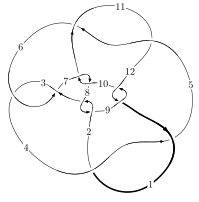
\includegraphics[width=112pt]{../../../GIT/diagram.site/Diagrams/png/1925_12a_1124.png}\\
\ \ \ A knot diagram\footnotemark}&
\allowdisplaybreaks
\textbf{Linearized knot diagam} \\
\cline{2-2}
 &
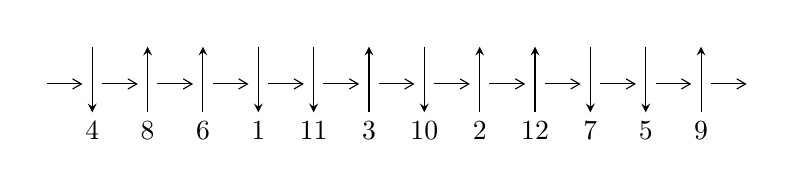
\begin{tikzpicture}[x=20pt, y=17pt]
	% nodes
	\node (C0) at (0, 0) {};
	\node (C1) at (1, 0) {};
	\node (C1U) at (1, +1) {};
	\node (C1D) at (1, -1) {4};

	\node (C2) at (2, 0) {};
	\node (C2U) at (2, +1) {};
	\node (C2D) at (2, -1) {8};

	\node (C3) at (3, 0) {};
	\node (C3U) at (3, +1) {};
	\node (C3D) at (3, -1) {6};

	\node (C4) at (4, 0) {};
	\node (C4U) at (4, +1) {};
	\node (C4D) at (4, -1) {1};

	\node (C5) at (5, 0) {};
	\node (C5U) at (5, +1) {};
	\node (C5D) at (5, -1) {11};

	\node (C6) at (6, 0) {};
	\node (C6U) at (6, +1) {};
	\node (C6D) at (6, -1) {3};

	\node (C7) at (7, 0) {};
	\node (C7U) at (7, +1) {};
	\node (C7D) at (7, -1) {10};

	\node (C8) at (8, 0) {};
	\node (C8U) at (8, +1) {};
	\node (C8D) at (8, -1) {2};

	\node (C9) at (9, 0) {};
	\node (C9U) at (9, +1) {};
	\node (C9D) at (9, -1) {12};

	\node (C10) at (10, 0) {};
	\node (C10U) at (10, +1) {};
	\node (C10D) at (10, -1) {7};

	\node (C11) at (11, 0) {};
	\node (C11U) at (11, +1) {};
	\node (C11D) at (11, -1) {5};

	\node (C12) at (12, 0) {};
	\node (C12U) at (12, +1) {};
	\node (C12D) at (12, -1) {9};
	\node (C13) at (13, 0) {};

	% arrows
	\draw[->,>={angle 60}]
	(C0) edge (C1) (C1) edge (C2) (C2) edge (C3) (C3) edge (C4) (C4) edge (C5) (C5) edge (C6) (C6) edge (C7) (C7) edge (C8) (C8) edge (C9) (C9) edge (C10) (C10) edge (C11) (C11) edge (C12) (C12) edge (C13) ;	\draw[->,>=stealth]
	(C1U) edge (C1D) (C2D) edge (C2U) (C3D) edge (C3U) (C4U) edge (C4D) (C5U) edge (C5D) (C6D) edge (C6U) (C7U) edge (C7D) (C8D) edge (C8U) (C9D) edge (C9U) (C10U) edge (C10D) (C11U) edge (C11D) (C12D) edge (C12U) ;
	\end{tikzpicture} \\
\hhline{~~} \\& 
\textbf{Solving Sequence} \\ \cline{2-2} 
 &
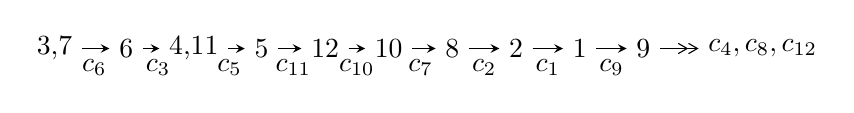
\begin{tikzpicture}[x=23pt, y=7pt]
	% node
	\node (A0) at (-1/8, 0) {3,7};
	\node (A1) at (1, 0) {6};
	\node (A2) at (33/16, 0) {4,11};
	\node (A3) at (25/8, 0) {5};
	\node (A4) at (33/8, 0) {12};
	\node (A5) at (41/8, 0) {10};
	\node (A6) at (49/8, 0) {8};
	\node (A7) at (57/8, 0) {2};
	\node (A8) at (65/8, 0) {1};
	\node (A9) at (73/8, 0) {9};
	\node (C1) at (1/2, -1) {$c_{6}$};
	\node (C2) at (3/2, -1) {$c_{3}$};
	\node (C3) at (21/8, -1) {$c_{5}$};
	\node (C4) at (29/8, -1) {$c_{11}$};
	\node (C5) at (37/8, -1) {$c_{10}$};
	\node (C6) at (45/8, -1) {$c_{7}$};
	\node (C7) at (53/8, -1) {$c_{2}$};
	\node (C8) at (61/8, -1) {$c_{1}$};
	\node (C9) at (69/8, -1) {$c_{9}$};
	\node (A10) at (11, 0) {$c_{4},c_{8},c_{12}$};

	% edge
	\draw[->,>=stealth]	
	(A0) edge (A1) (A1) edge (A2) (A2) edge (A3) (A3) edge (A4) (A4) edge (A5) (A5) edge (A6) (A6) edge (A7) (A7) edge (A8) (A8) edge (A9) ;
	\draw[->>,>={angle 60}]	
	(A9) edge (A10);
\end{tikzpicture} \\ 

\end{tabular} \\

\footnotetext{
The image of knot diagram is generated by the software ``\textbf{Draw programme}" developed by Andrew Bartholomew(\url{http://www.layer8.co.uk/maths/draw/index.htm\#Running-draw}), where we modified some parts for our purpose(\url{https://github.com/CATsTAILs/LinksPainter}).
}\phantom \\ \newline 
\centering \textbf{Ideals for irreducible components\footnotemark of $X_{\text{par}}$} 
 
\begin{align*}
I^u_{1}&=\langle 
1.07302\times10^{16} u^{25}+3.50154\times10^{16} u^{24}+\cdots+1.30132\times10^{17} b+3.86213\times10^{16},\\
\phantom{I^u_{1}}&\phantom{= \langle  }-3.50638\times10^{16} u^{25}-1.89759\times10^{17} u^{24}+\cdots+2.60265\times10^{17} a-6.11748\times10^{17},\;u^{26}+u^{25}+\cdots-14 u+3\rangle \\
I^u_{2}&=\langle 
-6.92061\times10^{445} u^{111}-1.24528\times10^{446} u^{110}+\cdots+3.50085\times10^{446} b-1.06405\times10^{447},\\
\phantom{I^u_{2}}&\phantom{= \langle  }-1.84028\times10^{450} u^{111}-2.50015\times10^{451} u^{110}+\cdots+2.82749\times10^{452} a-3.75263\times10^{453},\\
\phantom{I^u_{2}}&\phantom{= \langle  }u^{112}+2 u^{111}+\cdots+645 u+123\rangle \\
I^u_{3}&=\langle 
-8.60666\times10^{28} u^{35}+2.78547\times10^{29} u^{34}+\cdots+1.04041\times10^{29} b-4.59118\times10^{29},\\
\phantom{I^u_{3}}&\phantom{= \langle  }-2.41162\times10^{30} u^{35}+3.63435\times10^{31} u^{34}+\cdots+7.01535\times10^{30} a+6.17284\times10^{31},\;u^{36}-5 u^{35}+\cdots+3 u+1\rangle \\
I^u_{4}&=\langle 
b+u-1,\;a+1,\;u^2- u+1\rangle \\
\\
\end{align*}
\raggedright * 4 irreducible components of $\dim_{\mathbb{C}}=0$, with total 176 representations.\\
\footnotetext{All coefficients of polynomials are rational numbers. But the coefficients are sometimes approximated in decimal forms when there is not enough margin.}
\newpage
\renewcommand{\arraystretch}{1}
\centering \section*{I. $I^u_{1}= \langle 1.07\times10^{16} u^{25}+3.50\times10^{16} u^{24}+\cdots+1.30\times10^{17} b+3.86\times10^{16},\;-3.51\times10^{16} u^{25}-1.90\times10^{17} u^{24}+\cdots+2.60\times10^{17} a-6.12\times10^{17},\;u^{26}+u^{25}+\cdots-14 u+3 \rangle$}
\flushleft \textbf{(i) Arc colorings}\\
\begin{tabular}{m{7pt} m{180pt} m{7pt} m{180pt} }
\flushright $a_{3}=$&$\begin{pmatrix}0\\u\end{pmatrix}$ \\
\flushright $a_{7}=$&$\begin{pmatrix}1\\0\end{pmatrix}$ \\
\flushright $a_{6}=$&$\begin{pmatrix}1\\u^2\end{pmatrix}$ \\
\flushright $a_{4}=$&$\begin{pmatrix}u\\u^3+u\end{pmatrix}$ \\
\flushright $a_{11}=$&$\begin{pmatrix}0.134724 u^{25}+0.729100 u^{24}+\cdots-4.54509 u+2.35048\\-0.0824562 u^{25}-0.269075 u^{24}+\cdots+1.18090 u-0.296785\end{pmatrix}$ \\
\flushright $a_{5}=$&$\begin{pmatrix}-0.223395 u^{25}-0.761058 u^{24}+\cdots+4.15107 u-0.466322\\0.363051 u^{25}+0.387123 u^{24}+\cdots+2.48399 u-0.167850\end{pmatrix}$ \\
\flushright $a_{12}=$&$\begin{pmatrix}-0.517977 u^{25}+0.957739 u^{24}+\cdots-18.4642 u+4.40381\\-0.483957 u^{25}-0.564125 u^{24}+\cdots-1.03960 u-0.0706293\end{pmatrix}$ \\
\flushright $a_{10}=$&$\begin{pmatrix}0.0522675 u^{25}+0.460025 u^{24}+\cdots-3.36419 u+2.05370\\-0.0824562 u^{25}-0.269075 u^{24}+\cdots+1.18090 u-0.296785\end{pmatrix}$ \\
\flushright $a_{8}=$&$\begin{pmatrix}-0.0944248 u^{25}+0.107519 u^{24}+\cdots-3.24925 u+1.84810\\0.0343026 u^{25}-0.266952 u^{24}+\cdots+4.94697 u-1.34175\end{pmatrix}$ \\
\flushright $a_{2}=$&$\begin{pmatrix}0.396266 u^{25}+0.347145 u^{24}+\cdots-2.41543 u+0.113900\\-0.230814 u^{25}-0.152987 u^{24}+\cdots-2.28807 u+0.465361\end{pmatrix}$ \\
\flushright $a_{1}=$&$\begin{pmatrix}0.582885 u^{25}+0.580597 u^{24}+\cdots-0.964263 u-0.133469\\-0.0819378 u^{25}+0.0357949 u^{24}+\cdots-0.741099 u+0.0774950\end{pmatrix}$ \\
\flushright $a_{9}=$&$\begin{pmatrix}-1.42345 u^{25}-1.35854 u^{24}+\cdots-0.516330 u+0.499768\\-0.00228858 u^{25}-0.568183 u^{24}+\cdots+8.02692 u-1.74866\end{pmatrix}$\\&\end{tabular}
\flushleft \textbf{(ii) Obstruction class $= -1$}\\~\\
\flushleft \textbf{(iii) Cusp Shapes $= -\frac{50626243171306417}{43377435355664855} u^{25}-\frac{28511993568223339}{17350974142265942} u^{24}+\cdots-\frac{1992721032938816786}{43377435355664855} u+\frac{762069217574817183}{86754870711329710}$}\\~\\
\newpage\renewcommand{\arraystretch}{1}
\flushleft \textbf{(iv) u-Polynomials at the component}\newline \\
\begin{tabular}{m{50pt}|m{274pt}}
Crossings & \hspace{64pt}u-Polynomials at each crossing \\
\hline $$\begin{aligned}c_{1},c_{4},c_{7}\\c_{10}\end{aligned}$$&$\begin{aligned}
&u^{26}- u^{25}+\cdots+14 u+3
\end{aligned}$\\
\hline $$\begin{aligned}c_{2},c_{8}\end{aligned}$$&$\begin{aligned}
&4(4 u^{26}-36 u^{25}+\cdots-360 u+52)
\end{aligned}$\\
\hline $$\begin{aligned}c_{3},c_{6},c_{9}\\c_{12}\end{aligned}$$&$\begin{aligned}
&u^{26}+u^{25}+\cdots-14 u+3
\end{aligned}$\\
\hline $$\begin{aligned}c_{5},c_{11}\end{aligned}$$&$\begin{aligned}
&4(4 u^{26}+36 u^{25}+\cdots+360 u+52)
\end{aligned}$\\
\hline
\end{tabular}\\~\\
\newpage\renewcommand{\arraystretch}{1}
\flushleft \textbf{(v) Riley Polynomials at the component}\newline \\
\begin{tabular}{m{50pt}|m{274pt}}
Crossings & \hspace{64pt}Riley Polynomials at each crossing \\
\hline $$\begin{aligned}c_{1},c_{3},c_{4}\\c_{6},c_{7},c_{9}\\c_{10},c_{12}\end{aligned}$$&$\begin{aligned}
&y^{26}+9 y^{25}+\cdots+122 y+9
\end{aligned}$\\
\hline $$\begin{aligned}c_{2},c_{5},c_{8}\\c_{11}\end{aligned}$$&$\begin{aligned}
&16(16 y^{26}+8 y^{25}+\cdots+19952 y+2704)
\end{aligned}$\\
\hline
\end{tabular}\\~\\
\newpage\flushleft \textbf{(vi) Complex Volumes and Cusp Shapes}
$$\begin{array}{c|c|c}  
\text{Solutions to }I^u_{1}& \I (\text{vol} + \sqrt{-1}CS) & \text{Cusp shape}\\
 \hline 
\begin{aligned}
u &= \phantom{-}0.171905 + 1.015710 I \\
a &= -1.50278 + 0.45928 I \\
b &= \phantom{-}0.635907 - 0.179675 I\end{aligned}
 & -3.39880 + 2.53537 I & -6.23800 - 4.79646 I \\ \hline\begin{aligned}
u &= \phantom{-}0.171905 - 1.015710 I \\
a &= -1.50278 - 0.45928 I \\
b &= \phantom{-}0.635907 + 0.179675 I\end{aligned}
 & -3.39880 - 2.53537 I & -6.23800 + 4.79646 I \\ \hline\begin{aligned}
u &= -0.099111 + 0.948892 I \\
a &= \phantom{-}3.05682 + 0.16034 I \\
b &= -0.099111 - 0.948892 I\end{aligned}
 & \phantom{-0.000000 } -0.788870 I & \phantom{-0.000000 } 0. - 8.08674 I \\ \hline\begin{aligned}
u &= -0.099111 - 0.948892 I \\
a &= \phantom{-}3.05682 - 0.16034 I \\
b &= -0.099111 + 0.948892 I\end{aligned}
 & \phantom{-0.000000 -}0.788870 I & \phantom{-0.000000 -}0. + 8.08674 I \\ \hline\begin{aligned}
u &= -0.971898 + 0.533345 I \\
a &= \phantom{-}0.169703 - 0.026789 I \\
b &= -0.185899 + 1.252460 I\end{aligned}
 & \phantom{-}9.46539 + 0.44983 I & \phantom{-}9.20690 + 1.23580 I \\ \hline\begin{aligned}
u &= -0.971898 - 0.533345 I \\
a &= \phantom{-}0.169703 + 0.026789 I \\
b &= -0.185899 - 1.252460 I\end{aligned}
 & \phantom{-}9.46539 - 0.44983 I & \phantom{-}9.20690 - 1.23580 I \\ \hline\begin{aligned}
u &= \phantom{-}0.444034 + 1.042450 I \\
a &= \phantom{-}1.32030 + 0.64016 I \\
b &= -1.37806 - 0.69705 I\end{aligned}
 & -5.26475 + 4.42469 I & -3.07955 - 6.39392 I \\ \hline\begin{aligned}
u &= \phantom{-}0.444034 - 1.042450 I \\
a &= \phantom{-}1.32030 - 0.64016 I \\
b &= -1.37806 + 0.69705 I\end{aligned}
 & -5.26475 - 4.42469 I & -3.07955 + 6.39392 I \\ \hline\begin{aligned}
u &= \phantom{-}0.262934 + 0.820958 I \\
a &= -2.45447 - 0.41027 I \\
b &= \phantom{-}1.310570 + 0.212605 I\end{aligned}
 & -3.02770 + 1.50091 I & -0.38117 - 3.23499 I \\ \hline\begin{aligned}
u &= \phantom{-}0.262934 - 0.820958 I \\
a &= -2.45447 + 0.41027 I \\
b &= \phantom{-}1.310570 - 0.212605 I\end{aligned}
 & -3.02770 - 1.50091 I & -0.38117 + 3.23499 I\\
 \hline 
 \end{array}$$\newpage$$\begin{array}{c|c|c}  
\text{Solutions to }I^u_{1}& \I (\text{vol} + \sqrt{-1}CS) & \text{Cusp shape}\\
 \hline 
\begin{aligned}
u &= -0.185899 + 1.252460 I \\
a &= \phantom{-}0.863382 - 0.637518 I \\
b &= -0.971898 + 0.533345 I\end{aligned}
 & -9.46539 - 0.44983 I & -9.20690 - 1.23580 I \\ \hline\begin{aligned}
u &= -0.185899 - 1.252460 I \\
a &= \phantom{-}0.863382 + 0.637518 I \\
b &= -0.971898 - 0.533345 I\end{aligned}
 & -9.46539 + 0.44983 I & -9.20690 + 1.23580 I \\ \hline\begin{aligned}
u &= \phantom{-}0.462470 + 1.233400 I \\
a &= \phantom{-}1.380000 + 0.282313 I \\
b &= -0.568787 + 1.206040 I\end{aligned}
 & -4.58845 + 11.84040 I & -2.55501 - 8.84767 I \\ \hline\begin{aligned}
u &= \phantom{-}0.462470 - 1.233400 I \\
a &= \phantom{-}1.380000 - 0.282313 I \\
b &= -0.568787 - 1.206040 I\end{aligned}
 & -4.58845 - 11.84040 I & -2.55501 + 8.84767 I \\ \hline\begin{aligned}
u &= \phantom{-}1.310570 + 0.212605 I \\
a &= \phantom{-}0.222492 + 0.720110 I \\
b &= \phantom{-}0.262934 + 0.820958 I\end{aligned}
 & \phantom{-}3.02770 - 1.50091 I & \phantom{-}0.38117 + 3.23499 I \\ \hline\begin{aligned}
u &= \phantom{-}1.310570 - 0.212605 I \\
a &= \phantom{-}0.222492 - 0.720110 I \\
b &= \phantom{-}0.262934 - 0.820958 I\end{aligned}
 & \phantom{-}3.02770 + 1.50091 I & \phantom{-}0.38117 - 3.23499 I \\ \hline\begin{aligned}
u &= -0.568787 + 1.206040 I \\
a &= -1.61277 - 0.45045 I \\
b &= \phantom{-}0.462470 + 1.233400 I\end{aligned}
 & \phantom{-}4.58845 - 11.84040 I & \phantom{-}2.55501 + 8.84767 I \\ \hline\begin{aligned}
u &= -0.568787 - 1.206040 I \\
a &= -1.61277 + 0.45045 I \\
b &= \phantom{-}0.462470 - 1.233400 I\end{aligned}
 & \phantom{-}4.58845 + 11.84040 I & \phantom{-}2.55501 - 8.84767 I \\ \hline\begin{aligned}
u &= \phantom{-}0.635907 + 0.179675 I \\
a &= \phantom{-}0.28808 - 1.39043 I \\
b &= \phantom{-}0.171905 - 1.015710 I\end{aligned}
 & \phantom{-}3.39880 + 2.53537 I & \phantom{-}6.23800 - 4.79646 I \\ \hline\begin{aligned}
u &= \phantom{-}0.635907 - 0.179675 I \\
a &= \phantom{-}0.28808 + 1.39043 I \\
b &= \phantom{-}0.171905 + 1.015710 I\end{aligned}
 & \phantom{-}3.39880 - 2.53537 I & \phantom{-}6.23800 + 4.79646 I\\
 \hline 
 \end{array}$$\newpage$$\begin{array}{c|c|c}  
\text{Solutions to }I^u_{1}& \I (\text{vol} + \sqrt{-1}CS) & \text{Cusp shape}\\
 \hline 
\begin{aligned}
u &= -0.74288 + 1.31638 I \\
a &= \phantom{-}1.371160 + 0.094012 I \\
b &= -0.74288 - 1.31638 I\end{aligned}
 & \phantom{-0.000000 } -19.4256 I & \phantom{-0.000000 -}0. + 10.05625 I \\ \hline\begin{aligned}
u &= -0.74288 - 1.31638 I \\
a &= \phantom{-}1.371160 - 0.094012 I \\
b &= -0.74288 + 1.31638 I\end{aligned}
 & \phantom{-0.000000 -}19.4256 I & \phantom{-0.000000 } 0. - 10.05625 I \\ \hline\begin{aligned}
u &= -1.37806 + 0.69705 I \\
a &= -0.0055300 + 0.0592273 I \\
b &= \phantom{-}0.444034 - 1.042450 I\end{aligned}
 & \phantom{-}5.26475 + 4.42469 I & \phantom{-}3.07955 - 6.39392 I \\ \hline\begin{aligned}
u &= -1.37806 - 0.69705 I \\
a &= -0.0055300 - 0.0592273 I \\
b &= \phantom{-}0.444034 + 1.042450 I\end{aligned}
 & \phantom{-}5.26475 - 4.42469 I & \phantom{-}3.07955 + 6.39392 I \\ \hline\begin{aligned}
u &= \phantom{-}0.158808 + 0.320085 I \\
a &= \phantom{-}1.070290 + 0.730453 I \\
b &= \phantom{-}0.158808 - 0.320085 I\end{aligned}
 & \phantom{-0.000000 -}0.894091 I & \phantom{-0.000000 } 0. - 7.18165 I \\ \hline\begin{aligned}
u &= \phantom{-}0.158808 - 0.320085 I \\
a &= \phantom{-}1.070290 - 0.730453 I \\
b &= \phantom{-}0.158808 + 0.320085 I\end{aligned}
 & \phantom{-0.000000 } -0.894091 I & \phantom{-0.000000 -}0. + 7.18165 I\\
 \hline 
 \end{array}$$\newpage\newpage\renewcommand{\arraystretch}{1}
\centering \section*{II. $I^u_{2}= \langle -6.92\times10^{445} u^{111}-1.25\times10^{446} u^{110}+\cdots+3.50\times10^{446} b-1.06\times10^{447},\;-1.84\times10^{450} u^{111}-2.50\times10^{451} u^{110}+\cdots+2.83\times10^{452} a-3.75\times10^{453},\;u^{112}+2 u^{111}+\cdots+645 u+123 \rangle$}
\flushleft \textbf{(i) Arc colorings}\\
\begin{tabular}{m{7pt} m{180pt} m{7pt} m{180pt} }
\flushright $a_{3}=$&$\begin{pmatrix}0\\u\end{pmatrix}$ \\
\flushright $a_{7}=$&$\begin{pmatrix}1\\0\end{pmatrix}$ \\
\flushright $a_{6}=$&$\begin{pmatrix}1\\u^2\end{pmatrix}$ \\
\flushright $a_{4}=$&$\begin{pmatrix}u\\u^3+u\end{pmatrix}$ \\
\flushright $a_{11}=$&$\begin{pmatrix}0.00650853 u^{111}+0.0884229 u^{110}+\cdots+57.9641 u+13.2719\\0.197684 u^{111}+0.355707 u^{110}+\cdots+57.5559 u+3.03942\end{pmatrix}$ \\
\flushright $a_{5}=$&$\begin{pmatrix}0.101099 u^{111}+0.135504 u^{110}+\cdots-53.2054 u-12.7494\\-0.115566 u^{111}-0.291705 u^{110}+\cdots-127.776 u-20.8814\end{pmatrix}$ \\
\flushright $a_{12}=$&$\begin{pmatrix}-0.126207 u^{111}-0.259103 u^{110}+\cdots-76.2442 u-9.47282\\-0.294134 u^{111}-0.552574 u^{110}+\cdots-115.549 u-10.3189\end{pmatrix}$ \\
\flushright $a_{10}=$&$\begin{pmatrix}0.204192 u^{111}+0.444130 u^{110}+\cdots+115.520 u+16.3114\\0.197684 u^{111}+0.355707 u^{110}+\cdots+57.5559 u+3.03942\end{pmatrix}$ \\
\flushright $a_{8}=$&$\begin{pmatrix}0.0135688 u^{111}+0.103593 u^{110}+\cdots+88.4866 u+17.2247\\0.191731 u^{111}+0.377269 u^{110}+\cdots+96.3823 u+10.7157\end{pmatrix}$ \\
\flushright $a_{2}=$&$\begin{pmatrix}0.0751224 u^{111}+0.104048 u^{110}+\cdots-57.5579 u-15.7583\\0.0701494 u^{111}+0.0353507 u^{110}+\cdots-80.4689 u-20.2555\end{pmatrix}$ \\
\flushright $a_{1}=$&$\begin{pmatrix}0.0859122 u^{111}+0.169795 u^{110}+\cdots-5.67199 u-5.36633\\0.0636436 u^{111}+0.0485745 u^{110}+\cdots-58.3981 u-15.2962\end{pmatrix}$ \\
\flushright $a_{9}=$&$\begin{pmatrix}0.0189622 u^{111}+0.0594773 u^{110}+\cdots-27.3713 u-5.26515\\0.0833554 u^{111}+0.159039 u^{110}+\cdots+40.9020 u+4.95769\end{pmatrix}$\\&\end{tabular}
\flushleft \textbf{(ii) Obstruction class $= -1$}\\~\\
\flushleft \textbf{(iii) Cusp Shapes $= 0.332720 u^{111}+0.853504 u^{110}+\cdots+352.835 u+63.0911$}\\~\\
\newpage\renewcommand{\arraystretch}{1}
\flushleft \textbf{(iv) u-Polynomials at the component}\newline \\
\begin{tabular}{m{50pt}|m{274pt}}
Crossings & \hspace{64pt}u-Polynomials at each crossing \\
\hline $$\begin{aligned}c_{1},c_{4},c_{7}\\c_{10}\end{aligned}$$&$\begin{aligned}
&u^{112}-2 u^{111}+\cdots-645 u+123
\end{aligned}$\\
\hline $$\begin{aligned}c_{2},c_{8}\end{aligned}$$&$\begin{aligned}
&81(9 u^{56}+18 u^{55}+\cdots+784 u+455)^{2}
\end{aligned}$\\
\hline $$\begin{aligned}c_{3},c_{6},c_{9}\\c_{12}\end{aligned}$$&$\begin{aligned}
&u^{112}+2 u^{111}+\cdots+645 u+123
\end{aligned}$\\
\hline $$\begin{aligned}c_{5},c_{11}\end{aligned}$$&$\begin{aligned}
&81(9 u^{56}-18 u^{55}+\cdots-784 u+455)^{2}
\end{aligned}$\\
\hline
\end{tabular}\\~\\
\newpage\renewcommand{\arraystretch}{1}
\flushleft \textbf{(v) Riley Polynomials at the component}\newline \\
\begin{tabular}{m{50pt}|m{274pt}}
Crossings & \hspace{64pt}Riley Polynomials at each crossing \\
\hline $$\begin{aligned}c_{1},c_{3},c_{4}\\c_{6},c_{7},c_{9}\\c_{10},c_{12}\end{aligned}$$&$\begin{aligned}
&y^{112}+58 y^{111}+\cdots+478431 y+15129
\end{aligned}$\\
\hline $$\begin{aligned}c_{2},c_{5},c_{8}\\c_{11}\end{aligned}$$&$\begin{aligned}
&6561(81 y^{56}+3366 y^{55}+\cdots+2666804 y+207025)^{2}
\end{aligned}$\\
\hline
\end{tabular}\\~\\
\newpage\flushleft \textbf{(vi) Complex Volumes and Cusp Shapes}
$$\begin{array}{c|c|c}  
\text{Solutions to }I^u_{2}& \I (\text{vol} + \sqrt{-1}CS) & \text{Cusp shape}\\
 \hline 
\begin{aligned}
u &= \phantom{-}0.884165 + 0.446342 I \\
a &= \phantom{-}0.105843 - 0.289868 I \\
b &= -0.528679 - 0.595350 I\end{aligned}
 & -1.47297 + 2.83228 I & \phantom{-0.000000 } 0 \\ \hline\begin{aligned}
u &= \phantom{-}0.884165 - 0.446342 I \\
a &= \phantom{-}0.105843 + 0.289868 I \\
b &= -0.528679 + 0.595350 I\end{aligned}
 & -1.47297 - 2.83228 I & \phantom{-0.000000 } 0 \\ \hline\begin{aligned}
u &= -0.759962 + 0.702616 I \\
a &= \phantom{-}0.087653 + 0.516964 I \\
b &= \phantom{-}0.47409 - 1.34478 I\end{aligned}
 & \phantom{-}4.44565 - 1.93679 I & \phantom{-0.000000 } 0 \\ \hline\begin{aligned}
u &= -0.759962 - 0.702616 I \\
a &= \phantom{-}0.087653 - 0.516964 I \\
b &= \phantom{-}0.47409 + 1.34478 I\end{aligned}
 & \phantom{-}4.44565 + 1.93679 I & \phantom{-0.000000 } 0 \\ \hline\begin{aligned}
u &= -0.083724 + 0.953094 I \\
a &= -1.50640 - 0.24056 I \\
b &= \phantom{-}0.632718 + 1.068020 I\end{aligned}
 & -1.14303 - 2.47132 I & \phantom{-0.000000 } 0 \\ \hline\begin{aligned}
u &= -0.083724 - 0.953094 I \\
a &= -1.50640 + 0.24056 I \\
b &= \phantom{-}0.632718 - 1.068020 I\end{aligned}
 & -1.14303 + 2.47132 I & \phantom{-0.000000 } 0 \\ \hline\begin{aligned}
u &= \phantom{-}0.953861 + 0.057825 I \\
a &= -0.0126888 - 0.0747161 I \\
b &= \phantom{-}0.110749 - 1.287230 I\end{aligned}
 & \phantom{-}4.95021 + 2.36997 I & \phantom{-0.000000 } 0 \\ \hline\begin{aligned}
u &= \phantom{-}0.953861 - 0.057825 I \\
a &= -0.0126888 + 0.0747161 I \\
b &= \phantom{-}0.110749 + 1.287230 I\end{aligned}
 & \phantom{-}4.95021 - 2.36997 I & \phantom{-0.000000 } 0 \\ \hline\begin{aligned}
u &= -0.603185 + 0.740197 I \\
a &= \phantom{-}1.223860 - 0.582290 I \\
b &= -0.631209 + 0.232434 I\end{aligned}
 & \phantom{-}4.95021 - 2.36997 I & \phantom{-0.000000 } 0 \\ \hline\begin{aligned}
u &= -0.603185 - 0.740197 I \\
a &= \phantom{-}1.223860 + 0.582290 I \\
b &= -0.631209 - 0.232434 I\end{aligned}
 & \phantom{-}4.95021 + 2.36997 I & \phantom{-0.000000 } 0\\
 \hline 
 \end{array}$$\newpage$$\begin{array}{c|c|c}  
\text{Solutions to }I^u_{2}& \I (\text{vol} + \sqrt{-1}CS) & \text{Cusp shape}\\
 \hline 
\begin{aligned}
u &= -0.813104 + 0.676150 I \\
a &= \phantom{-}0.326904 - 0.584359 I \\
b &= -0.651444 + 1.158900 I\end{aligned}
 & \phantom{-}6.37753 + 0.27406 I & \phantom{-0.000000 } 0 \\ \hline\begin{aligned}
u &= -0.813104 - 0.676150 I \\
a &= \phantom{-}0.326904 + 0.584359 I \\
b &= -0.651444 - 1.158900 I\end{aligned}
 & \phantom{-}6.37753 - 0.27406 I & \phantom{-0.000000 } 0 \\ \hline\begin{aligned}
u &= \phantom{-}0.292409 + 1.020680 I \\
a &= -1.58954 - 0.29311 I \\
b &= \phantom{-}1.51678 + 0.35730 I\end{aligned}
 & -3.79390 + 0.81802 I & \phantom{-0.000000 } 0 \\ \hline\begin{aligned}
u &= \phantom{-}0.292409 - 1.020680 I \\
a &= -1.58954 + 0.29311 I \\
b &= \phantom{-}1.51678 - 0.35730 I\end{aligned}
 & -3.79390 - 0.81802 I & \phantom{-0.000000 } 0 \\ \hline\begin{aligned}
u &= \phantom{-}0.505254 + 0.780652 I \\
a &= -0.068301 - 0.984122 I \\
b &= \phantom{-}0.113786 - 0.316141 I\end{aligned}
 & -1.14303 + 2.47132 I & \phantom{-0.000000 } 0 \\ \hline\begin{aligned}
u &= \phantom{-}0.505254 - 0.780652 I \\
a &= -0.068301 + 0.984122 I \\
b &= \phantom{-}0.113786 + 0.316141 I\end{aligned}
 & -1.14303 - 2.47132 I & \phantom{-0.000000 } 0 \\ \hline\begin{aligned}
u &= -0.592492 + 0.892812 I \\
a &= -1.53226 + 0.66927 I \\
b &= \phantom{-}0.877171 + 0.152656 I\end{aligned}
 & \phantom{-}0.67163 - 7.34051 I & \phantom{-0.000000 } 0 \\ \hline\begin{aligned}
u &= -0.592492 - 0.892812 I \\
a &= -1.53226 - 0.66927 I \\
b &= \phantom{-}0.877171 - 0.152656 I\end{aligned}
 & \phantom{-}0.67163 + 7.34051 I & \phantom{-0.000000 } 0 \\ \hline\begin{aligned}
u &= -0.844071 + 0.315454 I \\
a &= -0.206766 - 0.113144 I \\
b &= \phantom{-}0.228643 - 1.394900 I\end{aligned}
 & \phantom{-}7.35971 + 6.55125 I & \phantom{-0.000000 } 0 \\ \hline\begin{aligned}
u &= -0.844071 - 0.315454 I \\
a &= -0.206766 + 0.113144 I \\
b &= \phantom{-}0.228643 + 1.394900 I\end{aligned}
 & \phantom{-}7.35971 - 6.55125 I & \phantom{-0.000000 } 0\\
 \hline 
 \end{array}$$\newpage$$\begin{array}{c|c|c}  
\text{Solutions to }I^u_{2}& \I (\text{vol} + \sqrt{-1}CS) & \text{Cusp shape}\\
 \hline 
\begin{aligned}
u &= \phantom{-}0.877171 + 0.152656 I \\
a &= \phantom{-}0.588923 + 1.119460 I \\
b &= -0.592492 + 0.892812 I\end{aligned}
 & -0.67163 + 7.34051 I & \phantom{-0.000000 } 0 \\ \hline\begin{aligned}
u &= \phantom{-}0.877171 - 0.152656 I \\
a &= \phantom{-}0.588923 - 1.119460 I \\
b &= -0.592492 - 0.892812 I\end{aligned}
 & -0.67163 - 7.34051 I & \phantom{-0.000000 } 0 \\ \hline\begin{aligned}
u &= \phantom{-}0.867572 + 0.075937 I \\
a &= \phantom{-}0.500076 + 0.274476 I \\
b &= \phantom{-}0.191909 + 1.225350 I\end{aligned}
 & \phantom{-}3.62547 - 2.48438 I & \phantom{-0.000000 } 0 \\ \hline\begin{aligned}
u &= \phantom{-}0.867572 - 0.075937 I \\
a &= \phantom{-}0.500076 - 0.274476 I \\
b &= \phantom{-}0.191909 - 1.225350 I\end{aligned}
 & \phantom{-}3.62547 + 2.48438 I & \phantom{-0.000000 } 0 \\ \hline\begin{aligned}
u &= \phantom{-}0.382832 + 0.766047 I \\
a &= -1.97355 + 0.24792 I \\
b &= \phantom{-}0.025588 - 0.334898 I\end{aligned}
 & -3.62547 + 2.48438 I & \phantom{-0.000000 } 0 \\ \hline\begin{aligned}
u &= \phantom{-}0.382832 - 0.766047 I \\
a &= -1.97355 - 0.24792 I \\
b &= \phantom{-}0.025588 + 0.334898 I\end{aligned}
 & -3.62547 - 2.48438 I & \phantom{-0.000000 } 0 \\ \hline\begin{aligned}
u &= -0.301465 + 1.117770 I \\
a &= -1.140040 + 0.061054 I \\
b &= \phantom{-}0.542791 + 1.207620 I\end{aligned}
 & -1.47297 - 2.83228 I & \phantom{-0.000000 } 0 \\ \hline\begin{aligned}
u &= -0.301465 - 1.117770 I \\
a &= -1.140040 - 0.061054 I \\
b &= \phantom{-}0.542791 - 1.207620 I\end{aligned}
 & -1.47297 + 2.83228 I & \phantom{-0.000000 } 0 \\ \hline\begin{aligned}
u &= \phantom{-}1.122590 + 0.283421 I \\
a &= -0.068402 + 0.143669 I \\
b &= -0.485724 - 1.193430 I\end{aligned}
 & \phantom{-0.000000 } -5.88229 I & \phantom{-0.000000 } 0 \\ \hline\begin{aligned}
u &= \phantom{-}1.122590 - 0.283421 I \\
a &= -0.068402 - 0.143669 I \\
b &= -0.485724 + 1.193430 I\end{aligned}
 & \phantom{-0.000000 -}5.88229 I & \phantom{-0.000000 } 0\\
 \hline 
 \end{array}$$\newpage$$\begin{array}{c|c|c}  
\text{Solutions to }I^u_{2}& \I (\text{vol} + \sqrt{-1}CS) & \text{Cusp shape}\\
 \hline 
\begin{aligned}
u &= -0.420227 + 1.088870 I \\
a &= \phantom{-}1.27405 + 1.05522 I \\
b &= -0.394596 - 1.264030 I\end{aligned}
 & \phantom{-}3.52423 + 3.40169 I & \phantom{-0.000000 } 0 \\ \hline\begin{aligned}
u &= -0.420227 - 1.088870 I \\
a &= \phantom{-}1.27405 - 1.05522 I \\
b &= -0.394596 + 1.264030 I\end{aligned}
 & \phantom{-}3.52423 - 3.40169 I & \phantom{-0.000000 } 0 \\ \hline\begin{aligned}
u &= -0.637995 + 0.990357 I \\
a &= -1.68006 - 0.10686 I \\
b &= \phantom{-}0.75424 + 1.21771 I\end{aligned}
 & \phantom{-}3.52423 - 3.40169 I & \phantom{-0.000000 } 0 \\ \hline\begin{aligned}
u &= -0.637995 - 0.990357 I \\
a &= -1.68006 + 0.10686 I \\
b &= \phantom{-}0.75424 - 1.21771 I\end{aligned}
 & \phantom{-}3.52423 + 3.40169 I & \phantom{-0.000000 } 0 \\ \hline\begin{aligned}
u &= -0.354197 + 1.136970 I \\
a &= -1.32575 - 1.08797 I \\
b &= \phantom{-}0.585869 + 1.043190 I\end{aligned}
 & \phantom{-}4.44565 - 1.93679 I & \phantom{-0.000000 } 0 \\ \hline\begin{aligned}
u &= -0.354197 - 1.136970 I \\
a &= -1.32575 + 1.08797 I \\
b &= \phantom{-}0.585869 - 1.043190 I\end{aligned}
 & \phantom{-}4.44565 + 1.93679 I & \phantom{-0.000000 } 0 \\ \hline\begin{aligned}
u &= -0.462140 + 1.099560 I \\
a &= \phantom{-}1.42581 - 0.30656 I \\
b &= -0.685238 - 1.173630 I\end{aligned}
 & -7.35971 - 6.55125 I & \phantom{-0.000000 } 0 \\ \hline\begin{aligned}
u &= -0.462140 - 1.099560 I \\
a &= \phantom{-}1.42581 + 0.30656 I \\
b &= -0.685238 + 1.173630 I\end{aligned}
 & -7.35971 + 6.55125 I & \phantom{-0.000000 } 0 \\ \hline\begin{aligned}
u &= \phantom{-}0.585869 + 1.043190 I \\
a &= \phantom{-}0.473389 + 0.565880 I \\
b &= -0.354197 + 1.136970 I\end{aligned}
 & -4.44565 + 1.93679 I & \phantom{-0.000000 } 0 \\ \hline\begin{aligned}
u &= \phantom{-}0.585869 - 1.043190 I \\
a &= \phantom{-}0.473389 - 0.565880 I \\
b &= -0.354197 - 1.136970 I\end{aligned}
 & -4.44565 - 1.93679 I & \phantom{-0.000000 } 0\\
 \hline 
 \end{array}$$\newpage$$\begin{array}{c|c|c}  
\text{Solutions to }I^u_{2}& \I (\text{vol} + \sqrt{-1}CS) & \text{Cusp shape}\\
 \hline 
\begin{aligned}
u &= -1.194380 + 0.109868 I \\
a &= -0.052951 + 1.071920 I \\
b &= \phantom{-}0.387030 + 0.624603 I\end{aligned}
 & \phantom{-}3.79390 + 0.81802 I & \phantom{-0.000000 } 0 \\ \hline\begin{aligned}
u &= -1.194380 - 0.109868 I \\
a &= -0.052951 - 1.071920 I \\
b &= \phantom{-}0.387030 - 0.624603 I\end{aligned}
 & \phantom{-}3.79390 - 0.81802 I & \phantom{-0.000000 } 0 \\ \hline\begin{aligned}
u &= -0.528679 + 0.595350 I \\
a &= -0.894547 + 0.830069 I \\
b &= \phantom{-}0.884165 - 0.446342 I\end{aligned}
 & \phantom{-}1.47297 + 2.83228 I & \phantom{-0.000000 } 0 \\ \hline\begin{aligned}
u &= -0.528679 - 0.595350 I \\
a &= -0.894547 - 0.830069 I \\
b &= \phantom{-}0.884165 + 0.446342 I\end{aligned}
 & \phantom{-}1.47297 - 2.83228 I & \phantom{-0.000000 } 0 \\ \hline\begin{aligned}
u &= -0.714680 + 1.010660 I \\
a &= \phantom{-}1.71981 - 0.07841 I \\
b &= -0.907798 - 0.937963 I\end{aligned}
 & \phantom{-}5.36521 - 6.00891 I & \phantom{-0.000000 } 0 \\ \hline\begin{aligned}
u &= -0.714680 - 1.010660 I \\
a &= \phantom{-}1.71981 + 0.07841 I \\
b &= -0.907798 + 0.937963 I\end{aligned}
 & \phantom{-}5.36521 + 6.00891 I & \phantom{-0.000000 } 0 \\ \hline\begin{aligned}
u &= \phantom{-}0.191909 + 1.225350 I \\
a &= -1.139030 + 0.218604 I \\
b &= \phantom{-}0.867572 + 0.075937 I\end{aligned}
 & -3.62547 + 2.48438 I & \phantom{-0.000000 } 0 \\ \hline\begin{aligned}
u &= \phantom{-}0.191909 - 1.225350 I \\
a &= -1.139030 - 0.218604 I \\
b &= \phantom{-}0.867572 - 0.075937 I\end{aligned}
 & -3.62547 - 2.48438 I & \phantom{-0.000000 } 0 \\ \hline\begin{aligned}
u &= \phantom{-}0.632718 + 1.068020 I \\
a &= \phantom{-}0.918916 - 0.125547 I \\
b &= -0.083724 + 0.953094 I\end{aligned}
 & \phantom{-}1.14303 + 2.47132 I & \phantom{-0.000000 } 0 \\ \hline\begin{aligned}
u &= \phantom{-}0.632718 - 1.068020 I \\
a &= \phantom{-}0.918916 + 0.125547 I \\
b &= -0.083724 - 0.953094 I\end{aligned}
 & \phantom{-}1.14303 - 2.47132 I & \phantom{-0.000000 } 0\\
 \hline 
 \end{array}$$\newpage$$\begin{array}{c|c|c}  
\text{Solutions to }I^u_{2}& \I (\text{vol} + \sqrt{-1}CS) & \text{Cusp shape}\\
 \hline 
\begin{aligned}
u &= \phantom{-}0.387030 + 0.624603 I \\
a &= \phantom{-}2.72128 + 0.74896 I \\
b &= -1.194380 + 0.109868 I\end{aligned}
 & -3.79390 - 0.81802 I & -3.81901 + 0.78619 I \\ \hline\begin{aligned}
u &= \phantom{-}0.387030 - 0.624603 I \\
a &= \phantom{-}2.72128 - 0.74896 I \\
b &= -1.194380 - 0.109868 I\end{aligned}
 & -3.79390 + 0.81802 I & -3.81901 - 0.78619 I \\ \hline\begin{aligned}
u &= -0.491811 + 1.165850 I \\
a &= \phantom{-}1.255800 - 0.397372 I \\
b &= -1.327960 + 0.393036 I\end{aligned}
 & -3.01787 - 12.23000 I & \phantom{-0.000000 } 0 \\ \hline\begin{aligned}
u &= -0.491811 - 1.165850 I \\
a &= \phantom{-}1.255800 + 0.397372 I \\
b &= -1.327960 - 0.393036 I\end{aligned}
 & -3.01787 + 12.23000 I & \phantom{-0.000000 } 0 \\ \hline\begin{aligned}
u &= -0.150119 + 0.718590 I \\
a &= -0.060211 - 0.683044 I \\
b &= -0.03391 + 1.85674 I\end{aligned}
 & \phantom{-}5.36521 - 6.00891 I & -5.23529 + 9.39142 I \\ \hline\begin{aligned}
u &= -0.150119 - 0.718590 I \\
a &= -0.060211 + 0.683044 I \\
b &= -0.03391 - 1.85674 I\end{aligned}
 & \phantom{-}5.36521 + 6.00891 I & -5.23529 - 9.39142 I \\ \hline\begin{aligned}
u &= -0.136237 + 0.713086 I \\
a &= -0.687415 + 0.337443 I \\
b &= \phantom{-}0.32677 - 1.66929 I\end{aligned}
 & \phantom{-}6.37753 - 0.27406 I & -3.16621 + 0.74603 I \\ \hline\begin{aligned}
u &= -0.136237 - 0.713086 I \\
a &= -0.687415 - 0.337443 I \\
b &= \phantom{-}0.32677 + 1.66929 I\end{aligned}
 & \phantom{-}6.37753 + 0.27406 I & -3.16621 - 0.74603 I \\ \hline\begin{aligned}
u &= -0.485724 + 1.193430 I \\
a &= -1.054970 + 0.157438 I \\
b &= \phantom{-}1.122590 - 0.283421 I\end{aligned}
 & \phantom{-0.000000 } -5.88229 I & \phantom{-0.000000 } 0 \\ \hline\begin{aligned}
u &= -0.485724 - 1.193430 I \\
a &= -1.054970 - 0.157438 I \\
b &= \phantom{-}1.122590 + 0.283421 I\end{aligned}
 & \phantom{-0.000000 -}5.88229 I & \phantom{-0.000000 } 0\\
 \hline 
 \end{array}$$\newpage$$\begin{array}{c|c|c}  
\text{Solutions to }I^u_{2}& \I (\text{vol} + \sqrt{-1}CS) & \text{Cusp shape}\\
 \hline 
\begin{aligned}
u &= -0.130420 + 0.698189 I \\
a &= \phantom{-}1.49124 + 0.08272 I \\
b &= -0.130420 - 0.698189 I\end{aligned}
 & \phantom{-0.000000 -}0.727774 I & \phantom{-0.000000 } 0. - 4.02174 I \\ \hline\begin{aligned}
u &= -0.130420 - 0.698189 I \\
a &= \phantom{-}1.49124 - 0.08272 I \\
b &= -0.130420 + 0.698189 I\end{aligned}
 & \phantom{-0.000000 } -0.727774 I & \phantom{-0.000000 -}0. + 4.02174 I \\ \hline\begin{aligned}
u &= \phantom{-}0.110749 + 1.287230 I \\
a &= -1.008870 + 0.047046 I \\
b &= \phantom{-}0.953861 - 0.057825 I\end{aligned}
 & -4.95021 + 2.36997 I & \phantom{-0.000000 } 0 \\ \hline\begin{aligned}
u &= \phantom{-}0.110749 - 1.287230 I \\
a &= -1.008870 - 0.047046 I \\
b &= \phantom{-}0.953861 + 0.057825 I\end{aligned}
 & -4.95021 - 2.36997 I & \phantom{-0.000000 } 0 \\ \hline\begin{aligned}
u &= -0.907798 + 0.937963 I \\
a &= \phantom{-}1.089720 - 0.578246 I \\
b &= -0.714680 - 1.010660 I\end{aligned}
 & -5.36521 - 6.00891 I & \phantom{-0.000000 } 0 \\ \hline\begin{aligned}
u &= -0.907798 - 0.937963 I \\
a &= \phantom{-}1.089720 + 0.578246 I \\
b &= -0.714680 + 1.010660 I\end{aligned}
 & -5.36521 + 6.00891 I & \phantom{-0.000000 } 0 \\ \hline\begin{aligned}
u &= \phantom{-}0.542791 + 1.207620 I \\
a &= \phantom{-}1.106730 - 0.527739 I \\
b &= -0.301465 + 1.117770 I\end{aligned}
 & \phantom{-}1.47297 + 2.83228 I & \phantom{-0.000000 } 0 \\ \hline\begin{aligned}
u &= \phantom{-}0.542791 - 1.207620 I \\
a &= \phantom{-}1.106730 + 0.527739 I \\
b &= -0.301465 - 1.117770 I\end{aligned}
 & \phantom{-}1.47297 - 2.83228 I & \phantom{-0.000000 } 0 \\ \hline\begin{aligned}
u &= -0.394596 + 1.264030 I \\
a &= \phantom{-}0.721570 - 0.337747 I \\
b &= -0.420227 - 1.088870 I\end{aligned}
 & -3.52423 + 3.40169 I & \phantom{-0.000000 } 0 \\ \hline\begin{aligned}
u &= -0.394596 - 1.264030 I \\
a &= \phantom{-}0.721570 + 0.337747 I \\
b &= -0.420227 + 1.088870 I\end{aligned}
 & -3.52423 - 3.40169 I & \phantom{-0.000000 } 0\\
 \hline 
 \end{array}$$\newpage$$\begin{array}{c|c|c}  
\text{Solutions to }I^u_{2}& \I (\text{vol} + \sqrt{-1}CS) & \text{Cusp shape}\\
 \hline 
\begin{aligned}
u &= -0.631209 + 0.232434 I \\
a &= -0.471205 + 0.855786 I \\
b &= -0.603185 + 0.740197 I\end{aligned}
 & -4.95021 + 2.36997 I & -5.26771 - 3.02633 I \\ \hline\begin{aligned}
u &= -0.631209 - 0.232434 I \\
a &= -0.471205 - 0.855786 I \\
b &= -0.603185 - 0.740197 I\end{aligned}
 & -4.95021 - 2.36997 I & -5.26771 + 3.02633 I \\ \hline\begin{aligned}
u &= -0.651444 + 1.158900 I \\
a &= \phantom{-}0.404280 - 0.334762 I \\
b &= -0.813104 + 0.676150 I\end{aligned}
 & -6.37753 - 0.27406 I & \phantom{-0.000000 } 0 \\ \hline\begin{aligned}
u &= -0.651444 - 1.158900 I \\
a &= \phantom{-}0.404280 + 0.334762 I \\
b &= -0.813104 - 0.676150 I\end{aligned}
 & -6.37753 + 0.27406 I & \phantom{-0.000000 } 0 \\ \hline\begin{aligned}
u &= \phantom{-}0.549092 + 1.229860 I \\
a &= -0.926899 - 0.049173 I \\
b &= \phantom{-}0.456838 - 1.292490 I\end{aligned}
 & -0.67163 + 7.34051 I & \phantom{-0.000000 } 0 \\ \hline\begin{aligned}
u &= \phantom{-}0.549092 - 1.229860 I \\
a &= -0.926899 + 0.049173 I \\
b &= \phantom{-}0.456838 + 1.292490 I\end{aligned}
 & -0.67163 - 7.34051 I & \phantom{-0.000000 } 0 \\ \hline\begin{aligned}
u &= -0.685238 + 1.173630 I \\
a &= \phantom{-}1.42898 + 0.26083 I \\
b &= -0.462140 - 1.099560 I\end{aligned}
 & \phantom{-}7.35971 - 6.55125 I & \phantom{-0.000000 } 0 \\ \hline\begin{aligned}
u &= -0.685238 - 1.173630 I \\
a &= \phantom{-}1.42898 - 0.26083 I \\
b &= -0.462140 + 1.099560 I\end{aligned}
 & \phantom{-}7.35971 + 6.55125 I & \phantom{-0.000000 } 0 \\ \hline\begin{aligned}
u &= -0.594063 + 0.232845 I \\
a &= -1.27489 + 2.45384 I \\
b &= -0.331498 + 0.096194 I\end{aligned}
 & \phantom{-}0.02827 - 8.03523 I & \phantom{-}1.79105 + 2.67120 I \\ \hline\begin{aligned}
u &= -0.594063 - 0.232845 I \\
a &= -1.27489 - 2.45384 I \\
b &= -0.331498 - 0.096194 I\end{aligned}
 & \phantom{-}0.02827 + 8.03523 I & \phantom{-}1.79105 - 2.67120 I\\
 \hline 
 \end{array}$$\newpage$$\begin{array}{c|c|c}  
\text{Solutions to }I^u_{2}& \I (\text{vol} + \sqrt{-1}CS) & \text{Cusp shape}\\
 \hline 
\begin{aligned}
u &= \phantom{-}0.456838 + 1.292490 I \\
a &= -1.242670 + 0.637725 I \\
b &= \phantom{-}0.549092 - 1.229860 I\end{aligned}
 & \phantom{-}0.67163 + 7.34051 I & \phantom{-0.000000 } 0 \\ \hline\begin{aligned}
u &= \phantom{-}0.456838 - 1.292490 I \\
a &= -1.242670 - 0.637725 I \\
b &= \phantom{-}0.549092 + 1.229860 I\end{aligned}
 & \phantom{-}0.67163 - 7.34051 I & \phantom{-0.000000 } 0 \\ \hline\begin{aligned}
u &= -1.327960 + 0.393036 I \\
a &= \phantom{-}0.0448775 - 0.0484661 I \\
b &= -0.491811 + 1.165850 I\end{aligned}
 & \phantom{-}3.01787 + 12.23000 I & \phantom{-0.000000 } 0 \\ \hline\begin{aligned}
u &= -1.327960 - 0.393036 I \\
a &= \phantom{-}0.0448775 + 0.0484661 I \\
b &= -0.491811 - 1.165850 I\end{aligned}
 & \phantom{-}3.01787 - 12.23000 I & \phantom{-0.000000 } 0 \\ \hline\begin{aligned}
u &= \phantom{-}0.228643 + 1.394900 I \\
a &= \phantom{-}0.841152 + 0.465681 I \\
b &= -0.844071 - 0.315454 I\end{aligned}
 & -7.35971 + 6.55125 I & \phantom{-0.000000 } 0 \\ \hline\begin{aligned}
u &= \phantom{-}0.228643 - 1.394900 I \\
a &= \phantom{-}0.841152 - 0.465681 I \\
b &= -0.844071 + 0.315454 I\end{aligned}
 & -7.35971 - 6.55125 I & \phantom{-0.000000 } 0 \\ \hline\begin{aligned}
u &= \phantom{-}0.47409 + 1.34478 I \\
a &= \phantom{-}0.641073 + 0.341067 I \\
b &= -0.759962 - 0.702616 I\end{aligned}
 & -4.44565 - 1.93679 I & \phantom{-0.000000 } 0 \\ \hline\begin{aligned}
u &= \phantom{-}0.47409 - 1.34478 I \\
a &= \phantom{-}0.641073 - 0.341067 I \\
b &= -0.759962 + 0.702616 I\end{aligned}
 & -4.44565 + 1.93679 I & \phantom{-0.000000 } 0 \\ \hline\begin{aligned}
u &= \phantom{-}0.60329 + 1.29581 I \\
a &= -1.204750 + 0.272854 I \\
b &= \phantom{-}0.62598 - 1.34876 I\end{aligned}
 & -0.02827 + 8.03523 I & \phantom{-0.000000 } 0 \\ \hline\begin{aligned}
u &= \phantom{-}0.60329 - 1.29581 I \\
a &= -1.204750 - 0.272854 I \\
b &= \phantom{-}0.62598 + 1.34876 I\end{aligned}
 & -0.02827 - 8.03523 I & \phantom{-0.000000 } 0\\
 \hline 
 \end{array}$$\newpage$$\begin{array}{c|c|c}  
\text{Solutions to }I^u_{2}& \I (\text{vol} + \sqrt{-1}CS) & \text{Cusp shape}\\
 \hline 
\begin{aligned}
u &= \phantom{-}0.67222 + 1.26173 I \\
a &= \phantom{-}1.46091 - 0.17983 I \\
b &= -0.82966 + 1.29407 I\end{aligned}
 & -3.01787 + 12.23000 I & \phantom{-0.000000 } 0 \\ \hline\begin{aligned}
u &= \phantom{-}0.67222 - 1.26173 I \\
a &= \phantom{-}1.46091 + 0.17983 I \\
b &= -0.82966 - 1.29407 I\end{aligned}
 & -3.01787 - 12.23000 I & \phantom{-0.000000 } 0 \\ \hline\begin{aligned}
u &= \phantom{-}0.75424 + 1.21771 I \\
a &= \phantom{-}1.152110 + 0.295229 I \\
b &= -0.637995 + 0.990357 I\end{aligned}
 & -3.52423 + 3.40169 I & \phantom{-0.000000 } 0 \\ \hline\begin{aligned}
u &= \phantom{-}0.75424 - 1.21771 I \\
a &= \phantom{-}1.152110 - 0.295229 I \\
b &= -0.637995 - 0.990357 I\end{aligned}
 & -3.52423 - 3.40169 I & \phantom{-0.000000 } 0 \\ \hline\begin{aligned}
u &= \phantom{-}0.62598 + 1.34876 I \\
a &= -1.149320 + 0.241382 I \\
b &= \phantom{-}0.60329 - 1.29581 I\end{aligned}
 & \phantom{-}0.02827 + 8.03523 I & \phantom{-0.000000 } 0 \\ \hline\begin{aligned}
u &= \phantom{-}0.62598 - 1.34876 I \\
a &= -1.149320 - 0.241382 I \\
b &= \phantom{-}0.60329 + 1.29581 I\end{aligned}
 & \phantom{-}0.02827 - 8.03523 I & \phantom{-0.000000 } 0 \\ \hline\begin{aligned}
u &= \phantom{-}0.407749 + 0.238643 I \\
a &= \phantom{-}0.256790 + 0.906420 I \\
b &= \phantom{-}0.407749 - 0.238643 I\end{aligned}
 & \phantom{-0.000000 -}0.727774 I & \phantom{-0.000000 } 0. - 4.02174 I \\ \hline\begin{aligned}
u &= \phantom{-}0.407749 - 0.238643 I \\
a &= \phantom{-}0.256790 - 0.906420 I \\
b &= \phantom{-}0.407749 + 0.238643 I\end{aligned}
 & \phantom{-0.000000 } -0.727774 I & \phantom{-0.000000 -}0. + 4.02174 I \\ \hline\begin{aligned}
u &= -0.82966 + 1.29407 I \\
a &= -1.191020 + 0.005097 I \\
b &= \phantom{-}0.67222 + 1.26173 I\end{aligned}
 & \phantom{-}3.01787 - 12.23000 I & \phantom{-0.000000 } 0 \\ \hline\begin{aligned}
u &= -0.82966 - 1.29407 I \\
a &= -1.191020 - 0.005097 I \\
b &= \phantom{-}0.67222 - 1.26173 I\end{aligned}
 & \phantom{-}3.01787 + 12.23000 I & \phantom{-0.000000 } 0\\
 \hline 
 \end{array}$$\newpage$$\begin{array}{c|c|c}  
\text{Solutions to }I^u_{2}& \I (\text{vol} + \sqrt{-1}CS) & \text{Cusp shape}\\
 \hline 
\begin{aligned}
u &= \phantom{-}1.51678 + 0.35730 I \\
a &= \phantom{-}0.0623760 + 0.0218971 I \\
b &= \phantom{-}0.292409 + 1.020680 I\end{aligned}
 & \phantom{-}3.79390 - 0.81802 I & \phantom{-0.000000 } 0 \\ \hline\begin{aligned}
u &= \phantom{-}1.51678 - 0.35730 I \\
a &= \phantom{-}0.0623760 - 0.0218971 I \\
b &= \phantom{-}0.292409 - 1.020680 I\end{aligned}
 & \phantom{-}3.79390 + 0.81802 I & \phantom{-0.000000 } 0 \\ \hline\begin{aligned}
u &= -0.331498 + 0.096194 I \\
a &= \phantom{-}2.52818 - 4.96451 I \\
b &= -0.594063 + 0.232845 I\end{aligned}
 & -0.02827 + 8.03523 I & -1.79105 - 2.67120 I \\ \hline\begin{aligned}
u &= -0.331498 - 0.096194 I \\
a &= \phantom{-}2.52818 + 4.96451 I \\
b &= -0.594063 - 0.232845 I\end{aligned}
 & -0.02827 - 8.03523 I & -1.79105 + 2.67120 I \\ \hline\begin{aligned}
u &= \phantom{-}0.113786 + 0.316141 I \\
a &= -2.78656 + 2.28051 I \\
b &= \phantom{-}0.505254 - 0.780652 I\end{aligned}
 & \phantom{-}1.14303 + 2.47132 I & \phantom{-}5.07801 - 4.40819 I \\ \hline\begin{aligned}
u &= \phantom{-}0.113786 - 0.316141 I \\
a &= -2.78656 - 2.28051 I \\
b &= \phantom{-}0.505254 + 0.780652 I\end{aligned}
 & \phantom{-}1.14303 - 2.47132 I & \phantom{-}5.07801 + 4.40819 I \\ \hline\begin{aligned}
u &= \phantom{-}0.025588 + 0.334898 I \\
a &= -4.37473 - 2.36208 I \\
b &= \phantom{-}0.382832 - 0.766047 I\end{aligned}
 & \phantom{-}3.62547 + 2.48438 I & \phantom{-}2.78870 - 4.88253 I \\ \hline\begin{aligned}
u &= \phantom{-}0.025588 - 0.334898 I \\
a &= -4.37473 + 2.36208 I \\
b &= \phantom{-}0.382832 + 0.766047 I\end{aligned}
 & \phantom{-}3.62547 - 2.48438 I & \phantom{-}2.78870 + 4.88253 I \\ \hline\begin{aligned}
u &= \phantom{-}0.32677 + 1.66929 I \\
a &= -0.156499 + 0.567736 I \\
b &= -0.136237 - 0.713086 I\end{aligned}
 & -6.37753 - 0.27406 I & \phantom{-0.000000 } 0 \\ \hline\begin{aligned}
u &= \phantom{-}0.32677 - 1.66929 I \\
a &= -0.156499 - 0.567736 I \\
b &= -0.136237 + 0.713086 I\end{aligned}
 & -6.37753 + 0.27406 I & \phantom{-0.000000 } 0\\
 \hline 
 \end{array}$$\newpage$$\begin{array}{c|c|c}  
\text{Solutions to }I^u_{2}& \I (\text{vol} + \sqrt{-1}CS) & \text{Cusp shape}\\
 \hline 
\begin{aligned}
u &= -0.03391 + 1.85674 I \\
a &= \phantom{-}0.123122 - 0.448880 I \\
b &= -0.150119 + 0.718590 I\end{aligned}
 & -5.36521 + 6.00891 I & \phantom{-0.000000 } 0 \\ \hline\begin{aligned}
u &= -0.03391 - 1.85674 I \\
a &= \phantom{-}0.123122 + 0.448880 I \\
b &= -0.150119 - 0.718590 I\end{aligned}
 & -5.36521 - 6.00891 I & \phantom{-0.000000 } 0\\
 \hline 
 \end{array}$$\newpage\newpage\renewcommand{\arraystretch}{1}
\centering \section*{III. $I^u_{3}= \langle -8.61\times10^{28} u^{35}+2.79\times10^{29} u^{34}+\cdots+1.04\times10^{29} b-4.59\times10^{29},\;-2.41\times10^{30} u^{35}+3.63\times10^{31} u^{34}+\cdots+7.02\times10^{30} a+6.17\times10^{31},\;u^{36}-5 u^{35}+\cdots+3 u+1 \rangle$}
\flushleft \textbf{(i) Arc colorings}\\
\begin{tabular}{m{7pt} m{180pt} m{7pt} m{180pt} }
\flushright $a_{3}=$&$\begin{pmatrix}0\\u\end{pmatrix}$ \\
\flushright $a_{7}=$&$\begin{pmatrix}1\\0\end{pmatrix}$ \\
\flushright $a_{6}=$&$\begin{pmatrix}1\\u^2\end{pmatrix}$ \\
\flushright $a_{4}=$&$\begin{pmatrix}u\\u^3+u\end{pmatrix}$ \\
\flushright $a_{11}=$&$\begin{pmatrix}0.343763 u^{35}-5.18057 u^{34}+\cdots-35.9438 u-8.79905\\0.827236 u^{35}-2.67728 u^{34}+\cdots+19.1420 u+4.41284\end{pmatrix}$ \\
\flushright $a_{5}=$&$\begin{pmatrix}-1.97717 u^{35}+9.97818 u^{34}+\cdots-3.34201 u-1.59573\\-0.413987 u^{35}+1.85894 u^{34}+\cdots-1.49699 u+2.12131\end{pmatrix}$ \\
\flushright $a_{12}=$&$\begin{pmatrix}2.20740 u^{35}-10.8526 u^{34}+\cdots+7.07737 u+0.548090\\-0.819026 u^{35}+4.38146 u^{34}+\cdots-5.54503 u-1.52076\end{pmatrix}$ \\
\flushright $a_{10}=$&$\begin{pmatrix}1.17100 u^{35}-7.85785 u^{34}+\cdots-16.8018 u-4.38620\\0.827236 u^{35}-2.67728 u^{34}+\cdots+19.1420 u+4.41284\end{pmatrix}$ \\
\flushright $a_{8}=$&$\begin{pmatrix}0.0970879 u^{35}+0.361789 u^{34}+\cdots+10.5563 u+4.13110\\0.224099 u^{35}-1.20829 u^{34}+\cdots-1.18107 u-3.05633\end{pmatrix}$ \\
\flushright $a_{2}=$&$\begin{pmatrix}0.258655 u^{35}-0.938548 u^{34}+\cdots-1.61611 u+0.482228\\0.912207 u^{35}-4.34155 u^{34}+\cdots+9.55551 u+0.0449479\end{pmatrix}$ \\
\flushright $a_{1}=$&$\begin{pmatrix}0.389085 u^{35}-1.76419 u^{34}+\cdots-2.58230 u+0.517489\\0.956784 u^{35}-4.62078 u^{34}+\cdots+8.97936 u+0.253698\end{pmatrix}$ \\
\flushright $a_{9}=$&$\begin{pmatrix}-0.429002 u^{35}+2.36713 u^{34}+\cdots+1.32597 u+2.11288\\1.00044 u^{35}-4.55551 u^{34}+\cdots+10.9307 u-0.129685\end{pmatrix}$\\&\end{tabular}
\flushleft \textbf{(ii) Obstruction class $= 1$}\\~\\
\flushleft \textbf{(iii) Cusp Shapes $= 0.329196 u^{35}+5.91364 u^{34}+\cdots+69.4025 u+25.0741$}\\~\\
\newpage\renewcommand{\arraystretch}{1}
\flushleft \textbf{(iv) u-Polynomials at the component}\newline \\
\begin{tabular}{m{50pt}|m{274pt}}
Crossings & \hspace{64pt}u-Polynomials at each crossing \\
\hline $$\begin{aligned}c_{1},c_{6},c_{7}\\c_{12}\end{aligned}$$&$\begin{aligned}
&u^{36}-5 u^{35}+\cdots+3 u+1
\end{aligned}$\\
\hline $$\begin{aligned}c_{2},c_{5},c_{8}\\c_{11}\end{aligned}$$&$\begin{aligned}
&64(64 u^{36}+848 u^{34}+\cdots+672 u^2+49)
\end{aligned}$\\
\hline $$\begin{aligned}c_{3},c_{4},c_{9}\\c_{10}\end{aligned}$$&$\begin{aligned}
&u^{36}+5 u^{35}+\cdots-3 u+1
\end{aligned}$\\
\hline
\end{tabular}\\~\\
\newpage\renewcommand{\arraystretch}{1}
\flushleft \textbf{(v) Riley Polynomials at the component}\newline \\
\begin{tabular}{m{50pt}|m{274pt}}
Crossings & \hspace{64pt}Riley Polynomials at each crossing \\
\hline $$\begin{aligned}c_{1},c_{3},c_{4}\\c_{6},c_{7},c_{9}\\c_{10},c_{12}\end{aligned}$$&$\begin{aligned}
&y^{36}+15 y^{35}+\cdots+19 y+1
\end{aligned}$\\
\hline $$\begin{aligned}c_{2},c_{5},c_{8}\\c_{11}\end{aligned}$$&$\begin{aligned}
&4096(64 y^{18}+848 y^{17}+\cdots+672 y+49)^{2}
\end{aligned}$\\
\hline
\end{tabular}\\~\\
\newpage\flushleft \textbf{(vi) Complex Volumes and Cusp Shapes}
$$\begin{array}{c|c|c}  
\text{Solutions to }I^u_{3}& \I (\text{vol} + \sqrt{-1}CS) & \text{Cusp shape}\\
 \hline 
\begin{aligned}
u &= -0.820724 + 0.538227 I \\
a &= -0.119632 + 0.530996 I \\
b &= \phantom{-}0.473731 - 1.205330 I\end{aligned}
 & \phantom{-}7.14238 + 0.08114 I & \phantom{-}7.67724 + 1.23653 I \\ \hline\begin{aligned}
u &= -0.820724 - 0.538227 I \\
a &= -0.119632 - 0.530996 I \\
b &= \phantom{-}0.473731 + 1.205330 I\end{aligned}
 & \phantom{-}7.14238 - 0.08114 I & \phantom{-}7.67724 - 1.23653 I \\ \hline\begin{aligned}
u &= \phantom{-}0.007256 + 0.938273 I \\
a &= -1.72452 - 0.81856 I \\
b &= \phantom{-}0.490597 + 0.946124 I\end{aligned}
 & \phantom{-0.000000 } -1.96250 I & \phantom{-0.000000 -}0. + 2.64993 I \\ \hline\begin{aligned}
u &= \phantom{-}0.007256 - 0.938273 I \\
a &= -1.72452 + 0.81856 I \\
b &= \phantom{-}0.490597 - 0.946124 I\end{aligned}
 & \phantom{-0.000000 -}1.96250 I & \phantom{-0.000000 } 0. - 2.64993 I \\ \hline\begin{aligned}
u &= \phantom{-}0.490597 + 0.946124 I \\
a &= \phantom{-}1.019180 + 0.392510 I \\
b &= \phantom{-}0.007256 + 0.938273 I\end{aligned}
 & \phantom{-0.000000 -}1.96250 I & \phantom{-0.000000 } 0. - 2.64993 I \\ \hline\begin{aligned}
u &= \phantom{-}0.490597 - 0.946124 I \\
a &= \phantom{-}1.019180 - 0.392510 I \\
b &= \phantom{-}0.007256 - 0.938273 I\end{aligned}
 & \phantom{-0.000000 } -1.96250 I & \phantom{-0.000000 -}0. + 2.64993 I \\ \hline\begin{aligned}
u &= -0.882211 + 0.276225 I \\
a &= \phantom{-}1.16611 - 1.41086 I \\
b &= \phantom{-}0.151685 - 0.669452 I\end{aligned}
 & \phantom{-}4.45586 + 1.91497 I & \phantom{-}9.84662 - 2.65327 I \\ \hline\begin{aligned}
u &= -0.882211 - 0.276225 I \\
a &= \phantom{-}1.16611 + 1.41086 I \\
b &= \phantom{-}0.151685 + 0.669452 I\end{aligned}
 & \phantom{-}4.45586 - 1.91497 I & \phantom{-}9.84662 + 2.65327 I \\ \hline\begin{aligned}
u &= \phantom{-}0.248696 + 1.128430 I \\
a &= -1.51618 - 0.02715 I \\
b &= \phantom{-}1.351170 + 0.185322 I\end{aligned}
 & -4.45586 + 1.91497 I & -9.84662 - 2.65327 I \\ \hline\begin{aligned}
u &= \phantom{-}0.248696 - 1.128430 I \\
a &= -1.51618 + 0.02715 I \\
b &= \phantom{-}1.351170 - 0.185322 I\end{aligned}
 & -4.45586 - 1.91497 I & -9.84662 + 2.65327 I\\
 \hline 
 \end{array}$$\newpage$$\begin{array}{c|c|c}  
\text{Solutions to }I^u_{3}& \I (\text{vol} + \sqrt{-1}CS) & \text{Cusp shape}\\
 \hline 
\begin{aligned}
u &= \phantom{-}0.204788 + 0.730230 I \\
a &= -2.56341 - 0.14708 I \\
b &= \phantom{-}1.303390 + 0.199477 I\end{aligned}
 & -2.85825\phantom{ +0.000000I} & \phantom{-}                -6
0.341175 + 0. 10   I\phantom{ +0.000000I} \\ \hline\begin{aligned}
u &= \phantom{-}0.204788 - 0.730230 I \\
a &= -2.56341 + 0.14708 I \\
b &= \phantom{-}1.303390 - 0.199477 I\end{aligned}
 & -2.85825\phantom{ +0.000000I} & \phantom{-}                -6
0.341175 + 0. 10   I\phantom{ +0.000000I} \\ \hline\begin{aligned}
u &= -0.684168 + 1.040190 I \\
a &= -1.66598 - 0.01887 I \\
b &= \phantom{-}0.829883 + 0.933923 I\end{aligned}
 & \phantom{-}5.78137 - 5.67225 I & \phantom{-}6.40075 + 0.51668 I \\ \hline\begin{aligned}
u &= -0.684168 - 1.040190 I \\
a &= -1.66598 + 0.01887 I \\
b &= \phantom{-}0.829883 - 0.933923 I\end{aligned}
 & \phantom{-}5.78137 + 5.67225 I & \phantom{-}6.40075 - 0.51668 I \\ \hline\begin{aligned}
u &= \phantom{-}0.829883 + 0.933923 I \\
a &= \phantom{-}1.096860 + 0.567991 I \\
b &= -0.684168 + 1.040190 I\end{aligned}
 & -5.78137 + 5.67225 I & -6.40075 - 0.51668 I \\ \hline\begin{aligned}
u &= \phantom{-}0.829883 - 0.933923 I \\
a &= \phantom{-}1.096860 - 0.567991 I \\
b &= -0.684168 - 1.040190 I\end{aligned}
 & -5.78137 - 5.67225 I & -6.40075 + 0.51668 I \\ \hline\begin{aligned}
u &= \phantom{-}0.473731 + 1.205330 I \\
a &= \phantom{-}0.514258 + 0.262124 I \\
b &= -0.820724 - 0.538227 I\end{aligned}
 & -7.14238 + 0.08114 I & -7.67724 + 1.23653 I \\ \hline\begin{aligned}
u &= \phantom{-}0.473731 - 1.205330 I \\
a &= \phantom{-}0.514258 - 0.262124 I \\
b &= -0.820724 + 0.538227 I\end{aligned}
 & -7.14238 - 0.08114 I & -7.67724 - 1.23653 I \\ \hline\begin{aligned}
u &= \phantom{-}0.151685 + 0.669452 I \\
a &= \phantom{-}3.31404 - 0.12734 I \\
b &= -0.882211 - 0.276225 I\end{aligned}
 & -4.45586 + 1.91497 I & -9.84662 - 2.65327 I \\ \hline\begin{aligned}
u &= \phantom{-}0.151685 - 0.669452 I \\
a &= \phantom{-}3.31404 + 0.12734 I \\
b &= -0.882211 + 0.276225 I\end{aligned}
 & -4.45586 - 1.91497 I & -9.84662 + 2.65327 I\\
 \hline 
 \end{array}$$\newpage$$\begin{array}{c|c|c}  
\text{Solutions to }I^u_{3}& \I (\text{vol} + \sqrt{-1}CS) & \text{Cusp shape}\\
 \hline 
\begin{aligned}
u &= \phantom{-}1.303390 + 0.199477 I \\
a &= \phantom{-}0.326461 + 0.647740 I \\
b &= \phantom{-}0.204788 + 0.730230 I\end{aligned}
 & \phantom{-}2.85825\phantom{ +0.000000I} & \phantom{-0.000000 } 0 \\ \hline\begin{aligned}
u &= \phantom{-}1.303390 - 0.199477 I \\
a &= \phantom{-}0.326461 - 0.647740 I \\
b &= \phantom{-}0.204788 - 0.730230 I\end{aligned}
 & \phantom{-}2.85825\phantom{ +0.000000I} & \phantom{-0.000000 } 0 \\ \hline\begin{aligned}
u &= -0.483298 + 0.463379 I \\
a &= \phantom{-}2.88275 - 2.52294 I \\
b &= -0.483298 - 0.463379 I\end{aligned}
 & \phantom{-0.000000 } -8.54028 I & \phantom{-0.000000 -}0. + 18.8239 I \\ \hline\begin{aligned}
u &= -0.483298 - 0.463379 I \\
a &= \phantom{-}2.88275 + 2.52294 I \\
b &= -0.483298 + 0.463379 I\end{aligned}
 & \phantom{-0.000000 -}8.54028 I & \phantom{-0.000000 } 0. - 18.8239 I \\ \hline\begin{aligned}
u &= \phantom{-}1.351170 + 0.185322 I \\
a &= \phantom{-}0.174105 + 0.084819 I \\
b &= \phantom{-}0.248696 + 1.128430 I\end{aligned}
 & \phantom{-}4.45586 - 1.91497 I & \phantom{-}9.84662 + 2.65327 I \\ \hline\begin{aligned}
u &= \phantom{-}1.351170 - 0.185322 I \\
a &= \phantom{-}0.174105 - 0.084819 I \\
b &= \phantom{-}0.248696 - 1.128430 I\end{aligned}
 & \phantom{-}4.45586 + 1.91497 I & \phantom{-}9.84662 - 2.65327 I \\ \hline\begin{aligned}
u &= \phantom{-}0.29330 + 1.41288 I \\
a &= \phantom{-}0.283615 - 0.183655 I \\
b &= -0.499882 - 0.217642 I\end{aligned}
 & -7.14238 - 0.08114 I & -7.67724 + 0. I\phantom{ +0.000000I} \\ \hline\begin{aligned}
u &= \phantom{-}0.29330 - 1.41288 I \\
a &= \phantom{-}0.283615 + 0.183655 I \\
b &= -0.499882 + 0.217642 I\end{aligned}
 & -7.14238 + 0.08114 I & -7.67724 + 0. I\phantom{ +0.000000I} \\ \hline\begin{aligned}
u &= -0.499882 + 0.217642 I \\
a &= \phantom{-}0.536918 + 1.080480 I \\
b &= \phantom{-}0.29330 - 1.41288 I\end{aligned}
 & \phantom{-}7.14238 - 0.08114 I & \phantom{-}7.67724 - 1.23653 I \\ \hline\begin{aligned}
u &= -0.499882 - 0.217642 I \\
a &= \phantom{-}0.536918 - 1.080480 I \\
b &= \phantom{-}0.29330 + 1.41288 I\end{aligned}
 & \phantom{-}7.14238 + 0.08114 I & \phantom{-}7.67724 + 1.23653 I\\
 \hline 
 \end{array}$$\newpage$$\begin{array}{c|c|c}  
\text{Solutions to }I^u_{3}& \I (\text{vol} + \sqrt{-1}CS) & \text{Cusp shape}\\
 \hline 
\begin{aligned}
u &= \phantom{-}0.55869 + 1.38511 I \\
a &= -1.074710 + 0.371738 I \\
b &= \phantom{-}0.55869 - 1.38511 I\end{aligned}
 & \phantom{-0.000000 -}8.54028 I & \phantom{-0.000000 } 0. - 18.8239 I \\ \hline\begin{aligned}
u &= \phantom{-}0.55869 - 1.38511 I \\
a &= -1.074710 - 0.371738 I \\
b &= \phantom{-}0.55869 + 1.38511 I\end{aligned}
 & \phantom{-0.000000 } -8.54028 I & \phantom{-0.000000 -}0. + 18.8239 I \\ \hline\begin{aligned}
u &= -0.057431 + 0.371950 I \\
a &= \phantom{-}0.46776 - 2.06740 I \\
b &= \phantom{-}0.01453 + 1.70811 I\end{aligned}
 & \phantom{-}5.78137 - 5.67225 I & \phantom{-}6.40075 + 0.51668 I \\ \hline\begin{aligned}
u &= -0.057431 - 0.371950 I \\
a &= \phantom{-}0.46776 + 2.06740 I \\
b &= \phantom{-}0.01453 - 1.70811 I\end{aligned}
 & \phantom{-}5.78137 + 5.67225 I & \phantom{-}6.40075 - 0.51668 I \\ \hline\begin{aligned}
u &= \phantom{-}0.01453 + 1.70811 I \\
a &= -0.1176210 + 0.0610212 I \\
b &= -0.057431 + 0.371950 I\end{aligned}
 & -5.78137 + 5.67225 I & \phantom{-0.000000 } 0 \\ \hline\begin{aligned}
u &= \phantom{-}0.01453 - 1.70811 I \\
a &= -0.1176210 - 0.0610212 I \\
b &= -0.057431 - 0.371950 I\end{aligned}
 & -5.78137 - 5.67225 I & \phantom{-0.000000 } 0\\
 \hline 
 \end{array}$$\newpage\newpage\renewcommand{\arraystretch}{1}
\centering \section*{IV. $I^u_{4}= \langle b+u-1,\;a+1,\;u^2- u+1 \rangle$}
\flushleft \textbf{(i) Arc colorings}\\
\begin{tabular}{m{7pt} m{180pt} m{7pt} m{180pt} }
\flushright $a_{3}=$&$\begin{pmatrix}0\\u\end{pmatrix}$ \\
\flushright $a_{7}=$&$\begin{pmatrix}1\\0\end{pmatrix}$ \\
\flushright $a_{6}=$&$\begin{pmatrix}1\\u-1\end{pmatrix}$ \\
\flushright $a_{4}=$&$\begin{pmatrix}u\\u-1\end{pmatrix}$ \\
\flushright $a_{11}=$&$\begin{pmatrix}-1\\- u+1\end{pmatrix}$ \\
\flushright $a_{5}=$&$\begin{pmatrix}1\\u-1\end{pmatrix}$ \\
\flushright $a_{12}=$&$\begin{pmatrix}-1\\- u+1\end{pmatrix}$ \\
\flushright $a_{10}=$&$\begin{pmatrix}- u\\- u+1\end{pmatrix}$ \\
\flushright $a_{8}=$&$\begin{pmatrix}0\\- u\end{pmatrix}$ \\
\flushright $a_{2}=$&$\begin{pmatrix}0\\u\end{pmatrix}$ \\
\flushright $a_{1}=$&$\begin{pmatrix}-1\\0\end{pmatrix}$ \\
\flushright $a_{9}=$&$\begin{pmatrix}0\\- u\end{pmatrix}$\\&\end{tabular}
\flushleft \textbf{(ii) Obstruction class $= 1$}\\~\\
\flushleft \textbf{(iii) Cusp Shapes $= -8 u+4$}\\~\\
\newpage\renewcommand{\arraystretch}{1}
\flushleft \textbf{(iv) u-Polynomials at the component}\newline \\
\begin{tabular}{m{50pt}|m{274pt}}
Crossings & \hspace{64pt}u-Polynomials at each crossing \\
\hline $$\begin{aligned}c_{1},c_{6},c_{7}\\c_{12}\end{aligned}$$&$\begin{aligned}
&u^2- u+1
\end{aligned}$\\
\hline $$\begin{aligned}c_{2},c_{5},c_{8}\\c_{11}\end{aligned}$$&$\begin{aligned}
&u^2
\end{aligned}$\\
\hline $$\begin{aligned}c_{3},c_{4},c_{9}\\c_{10}\end{aligned}$$&$\begin{aligned}
&u^2+u+1
\end{aligned}$\\
\hline
\end{tabular}\\~\\
\newpage\renewcommand{\arraystretch}{1}
\flushleft \textbf{(v) Riley Polynomials at the component}\newline \\
\begin{tabular}{m{50pt}|m{274pt}}
Crossings & \hspace{64pt}Riley Polynomials at each crossing \\
\hline $$\begin{aligned}c_{1},c_{3},c_{4}\\c_{6},c_{7},c_{9}\\c_{10},c_{12}\end{aligned}$$&$\begin{aligned}
&y^2+y+1
\end{aligned}$\\
\hline $$\begin{aligned}c_{2},c_{5},c_{8}\\c_{11}\end{aligned}$$&$\begin{aligned}
&y^2
\end{aligned}$\\
\hline
\end{tabular}\\~\\
\newpage\flushleft \textbf{(vi) Complex Volumes and Cusp Shapes}
$$\begin{array}{c|c|c}  
\text{Solutions to }I^u_{4}& \I (\text{vol} + \sqrt{-1}CS) & \text{Cusp shape}\\
 \hline 
\begin{aligned}
u &= \phantom{-}0.500000 + 0.866025 I \\
a &= -1.00000\phantom{ +0.000000I} \\
b &= \phantom{-}0.500000 - 0.866025 I\end{aligned}
 & \phantom{-0.000000 -}4.05977 I & \phantom{-0.000000 } 0. - 6.92820 I \\ \hline\begin{aligned}
u &= \phantom{-}0.500000 - 0.866025 I \\
a &= -1.00000\phantom{ +0.000000I} \\
b &= \phantom{-}0.500000 + 0.866025 I\end{aligned}
 & \phantom{-0.000000 } -4.05977 I & \phantom{-0.000000 -}0. + 6.92820 I\\
 \hline 
 \end{array}$$\newpage
\newpage\renewcommand{\arraystretch}{1}
\centering \section*{ V. u-Polynomials}
\begin{tabular}{m{50pt}|m{274pt}}
Crossings & \hspace{64pt}u-Polynomials at each crossing \\
\hline $$\begin{aligned}c_{1},c_{7}\end{aligned}$$&$\begin{aligned}
&(u^2- u+1)(u^{26}- u^{25}+\cdots+14 u+3)(u^{36}-5 u^{35}+\cdots+3 u+1)\\
&\cdot(u^{112}-2 u^{111}+\cdots-645 u+123)
\end{aligned}$\\
\hline $$\begin{aligned}c_{2},c_{8}\end{aligned}$$&$\begin{aligned}
&20736u^2(4 u^{26}-36 u^{25}+\cdots-360 u+52)\\
&\cdot(64 u^{36}+848 u^{34}+\cdots+672 u^2+49)\\
&\cdot(9 u^{56}+18 u^{55}+\cdots+784 u+455)^{2}
\end{aligned}$\\
\hline $$\begin{aligned}c_{3},c_{9}\end{aligned}$$&$\begin{aligned}
&(u^2+u+1)(u^{26}+u^{25}+\cdots-14 u+3)(u^{36}+5 u^{35}+\cdots-3 u+1)\\
&\cdot(u^{112}+2 u^{111}+\cdots+645 u+123)
\end{aligned}$\\
\hline $$\begin{aligned}c_{4},c_{10}\end{aligned}$$&$\begin{aligned}
&(u^2+u+1)(u^{26}- u^{25}+\cdots+14 u+3)(u^{36}+5 u^{35}+\cdots-3 u+1)\\
&\cdot(u^{112}-2 u^{111}+\cdots-645 u+123)
\end{aligned}$\\
\hline $$\begin{aligned}c_{5},c_{11}\end{aligned}$$&$\begin{aligned}
&20736u^2(4 u^{26}+36 u^{25}+\cdots+360 u+52)\\
&\cdot(64 u^{36}+848 u^{34}+\cdots+672 u^2+49)\\
&\cdot(9 u^{56}-18 u^{55}+\cdots-784 u+455)^{2}
\end{aligned}$\\
\hline $$\begin{aligned}c_{6},c_{12}\end{aligned}$$&$\begin{aligned}
&(u^2- u+1)(u^{26}+u^{25}+\cdots-14 u+3)(u^{36}-5 u^{35}+\cdots+3 u+1)\\
&\cdot(u^{112}+2 u^{111}+\cdots+645 u+123)
\end{aligned}$\\
\hline
\end{tabular}\newpage\renewcommand{\arraystretch}{1}
\centering \section*{ VI. Riley Polynomials}
\begin{tabular}{m{50pt}|m{274pt}}
Crossings & \hspace{64pt}Riley Polynomials at each crossing \\
\hline $$\begin{aligned}c_{1},c_{3},c_{4}\\c_{6},c_{7},c_{9}\\c_{10},c_{12}\end{aligned}$$&$\begin{aligned}
&(y^2+y+1)(y^{26}+9 y^{25}+\cdots+122 y+9)(y^{36}+15 y^{35}+\cdots+19 y+1)\\
&\cdot(y^{112}+58 y^{111}+\cdots+478431 y+15129)
\end{aligned}$\\
\hline $$\begin{aligned}c_{2},c_{5},c_{8}\\c_{11}\end{aligned}$$&$\begin{aligned}
&429981696y^2(64 y^{18}+848 y^{17}+\cdots+672 y+49)^{2}\\
&\cdot(16 y^{26}+8 y^{25}+\cdots+19952 y+2704)\\
&\cdot(81 y^{56}+3366 y^{55}+\cdots+2666804 y+207025)^{2}
\end{aligned}$\\
\hline
\end{tabular}
\vskip 2pc
\end{document}